\documentclass[12pt, oneside, a4paper, brazil]{abntex2}

\usepackage{uarial}
\usepackage[T1]{fontenc}
\usepackage[utf8]{inputenc}
\usepackage{indentfirst}
\usepackage{color}
\usepackage{graphicx}
\usepackage{microtype}
\usepackage[brazilian,hyperpageref]{backref}
\usepackage[alf]{abntex2cite}
\usepackage[table]{xcolor}

\renewcommand{\backrefpagesname}{Citado na(s) página(s):~}
\renewcommand{\backref}{}
\renewcommand*{\backrefalt}[4]{
\ifcase #1 %
	Nenhuma citação no texto.%
\or %
 Citado na página #2.%
\else
	Citado #1 vezes nas páginas #2.%
\fi}%
\renewcommand*\familydefault{\sfdefault}

%Capa
\titulo{O Código da Felicidade \\
	\tiny A arte de desenvolver aplicações de alto valor agregado, \\
	     escaláveis e confiáveis... Sendo feliz durante sua construção.
}
\autor{Derotino Fraga da Silveira Junior}
\local{Brasil}
\data{2016}
\instituicao{%
  Instituto Educacional do Rio Grande do Sul - IERGS
  \par
  Elaboração do Projeto de Marketing Digital
  \par
  Professora Orientadora: Taís Garcia Teixeira}
\tipotrabalho{Projeto de Trabalho de Conclusão}

\preambulo{Projeto de implantação de estratégia de marketing para a Companhia de Processamento de Dados do Município de Porto Alegre - Procempa.}

\definecolor{blue}{RGB}{41,5,195}
\makeatletter
\hypersetup{
     	%pagebackref=true,
		pdftitle={\@title},
		pdfauthor={\@author},
    	pdfsubject={\imprimirpreambulo},
	    pdfcreator={LaTeX with abnTeX2},
		pdfkeywords={marketing}{redes sociais}{Procempa},
		colorlinks=true,       		% false: boxed links; true: colored links
    	linkcolor=blue,          	% color of internal links
    	citecolor=blue,        		% color of links to bibliography
    	filecolor=magenta,      		% color of file links
		urlcolor=blue,
		bookmarksdepth=4
}
\makeatother

\setlength{\parindent}{1.3cm}
\setlength{\parskip}{0.2cm}
\makeindex

\begin{document}
\selectlanguage{brazil}
\frenchspacing
\imprimircapa
\imprimirfolhaderosto
%\pdfbookmark[0]{\listfigurename}{lof}
%\listoffigures*
\cleardoublepage
\pdfbookmark[0]{\listtablename}{lot}
\listoftables*
\cleardoublepage
%\begin{siglas}
%  \item[ABNT] Associação Brasileira de Normas Técnicas
%  \item[abnTeX] ABsurdas Normas para TeX
%\end{siglas}

%\begin{simbolos}
%  \item[$ \Gamma $] Letra grega Gama
%  \item[$ \Lambda $] Lambda
%  \item[$ \zeta $] Letra grega minúscula zeta
%  \item[$ \in $] Pertence
%\end{simbolos}

\pdfbookmark[0]{\contentsname}{toc}
\tableofcontents*
\cleardoublepage

\textual

\chapter{Introdução}

No presente cenário de constante evolução tecnológica, recursos cada vez mais limitados e cidadãos melhor informados e com necessidades crescentes, a Tecnologia da Informação firmou-se como um papel de destaque no apoio do crescimento e resolução de problemas das grandes cidades pelo mundo.


Nos últimos anos a Companhia de Processamento de Dados do Município de Porto Alegre - Procempa - colocou em prática diversas estratégias com o fim de potencializar projetos de melhorias para o cidadão e otimização de processos para potencializar o investimento público e garantir a transparência em seus processo.


Por ser uma companhia inovadora desde seu nascimento, o capital intelectual presente atualmente tem propiciado a entrega constante e satisfatória de melhorias para a cidade. Na empresa a experiência de colaboradores de longa data foi mesclada com o dinamismo de novos empregados, aprovados em concurso público em 2014, criando um ambiente de mudanças e melhorias constantes.


O presente trabalho buscará demonstrar estratégias de disseminação deste capital de forma a fomentar criação de comunidades, a resolução de problemas do cidadão de forma colaborativa, bem como o incentivo a novos investimentos no setor de tecnologia na cidade.


\chapter{Justificativa}

A Companhia de Processamento de Dados do Município de Porto Alegre  - Procempa - foi fundada em 9 de setembro de 1977 e sempre foi reconhecida nacionalmente como referência em tecnologia das cidades. Em vários momentos a empresa ganhou renomados prêmios do setor tecnológico e foi expoente em tecnologias de ponta.
No ano de 2014 a empresa definiu uma estratégia de crescimento, juntamente com a administração municipal, planejando e colocando em prática diversas ações que a colocaram em situação de prontidão para o atual momento e para as crescentes inovações do mercado. As principais ações foram:

\begin{itemize}
\item Execução de concurso público com a contratação de mais de 100 novos funcionários;
\item Estruturação de processos internos de controle e administração, visando melhorias na gestão e transparência;
\item Estabelecimento de gestão por metas e indicadores;
\item Atualização das estruturas de suporte aos sistemas e servidores;
\item Reforma das instalações visando a agilidade e conforto dos funcionários e
\item Contratação de consultoria para apoiar a implantação de métodos ágeis.
\end{itemize}
Este cenário desenha-se perfeito para o início de uma estratégia de marketing para apoio a esta grande evolução e divulgação dos resultados obtidos com as estratégias. O foco destas estratégias será o fomento de soluções que possam ajudar a melhorar a vida do cidadão, seja fornecendo subsídios, como modelos, tecnologias, metodologias, etc, para novas \textit{startups} no município, seja fornecendo novos serviços diretamente aos cidadãos, para melhorar o seu dia a dia.
Estas estratégias irão se basear em mídias sociais, estratégias de divulgação de informações, incentivo a produção de conteúdo pelos colaboradores, participação em comunidades livres, fornecendo e recebendo apoio das mesmas.


\chapter{Objetivos}
\section{Objetivos Gerais}
Estabelecer estratégia de marketing digital que possibilite à Procempa - Companhia de Processamento de Dados do Município de Porto Alegre - projetar-se como uma referência em tecnologia e processos de construção de software. Através da utilização de canais digitais de apoio a comunidades de desenvolvimento e redes sociais, contribuir para o desenvolvimento da cidade e contribuir com a melhoria dos serviços aos cidadãos.

\section{Objetivos Específicos}
Os objetivos específicos deste planejamento são:
\begin{itemize}
\item Estabelecer estratégias e políticas institucionais de divulgação do trabalho tecnológico realizado na empresa;
\item Criar plano de comunicação com o foco divulgar os projetos, metodologia e tecnologias utilizadas;
\item Propor a utilização de ferramenta de blog a ser disponibilizado para os colaboradores, com foco na disseminação do conhecimento gerado pela empresa;
\item Elaborar plano de endo marketing para demonstrar aos colaboradores os avanços recentes da companhia, visão de futuro e estimulo a participação nas comunidades propostas por este planejamento;
\item Definir técnicas de palavras chave em mecanismos de busca para possibilitar uma boa colocação das informações geradas pela companhia;
\item Criar comunidade de código aberto no site github.com, a ser disponibilizado conforme as políticas definidas nas políticas institucionais, para estímulo da participação dos desenvolvedores em comunidades de software livre;
\item Desenvolver comunidades focadas nas tecnologias que sustentam a cidade, com o uso estruturado das redes sociais e a interação com outro polos e estruturas com o mesmo fim. Estas comunidades seriam criadas através das redes sociais Facebook e Twitter;
\item Demonstrar formato de utilização da rede social stackoverflow.com como forma de absorção e disseminação de conhecimento;
\item Planejar indicadores que demonstrem a efetividade das ações em relação às estratégias da companhia;
\end{itemize}


\chapter{Metodologia da Pesquisa}

O trabalho será conduzido a partir das referências bibliográficas e com a utilização da metodologia Design thinking, proposta por \citeonline{Brown2010}:
\begin{citacao}
O design thinking evoluiu de um início modesto: artífices como William Morris, arquitetos como Frank Lloyd Wright e \textit{designers} industriais como Henry Dreyfuss e Ray e Charles Eames desejavam tornar o mundo mas acessível, belo e significativo.
\end{citacao}

Assim este trabalho seguirá de forma a buscar incessantemente a inovação e tornar o ecossistema da companhia melhor, com alguns passos propostos por \citeonline{Brown2010}:

\begin{citacao}
\begin{itemize}
\item \textbf{Comece pelo início}: O design thinking começa com a divergência, a tentativa deliberada de expandir a variedade de opções ao invés de restringí-las.
\item \textbf{Assuma uma abordagem centrada no ser humano}: Como o design thinking equilibra as perspectivas do usuário, da tecnologia e dos negócios, é, por natureza, integrador. Como ponto de partida, contudo, ele privilegia o usuário final.
\item \textbf{Fracasse logo, fracasse com frequência}: O tempo até o primeiro protótipo é um bom indicativo da vitalidade de uma cultura de inovação. Com que rapidez as ideias são elaboradas de forma tangível, de modo que possam ser testadas e melhoradas? Os líderes devem incentivar a experimentação e aceitar que não há nada de errado com o fracasso, contanto que ele ocorra no começo e se torne fonte de aprendizado.
\item \textbf{Procure ajuda profissional}: Eu não corto meu próprio cabelo nem troco o óleo do meu carro, embora, provavelmente, seja capaz disto. Em certas ocasiões, faz mais sentido sair de sua organização e buscar oportunidades de expandir o ecossistema de inovação.
\item \textbf{Compartilhe a inspiração}: Não esqueça sua rede interna. Grande parte dos esforços relativos ao compartilhamento de conhecimento ao longo da última década se concentrou na eficiência. Talvez seja a hora de pensar em como suas redes de conhecimento sustentam a \emph{inspiração}.
\end{itemize}
\end{citacao}
Com estes e outros preceitos iremos buscar um trabalho divertido e inovador sempre pensando na companhia como parte de um grande sistema que de acordo com \citeonline{Brown2010} "Aos pensar em função do sistema como um todo as empresas podem se beneficiar de melhores oportunidades" .


\chapter{Referencial Teórico}

Vivemos atualmente a era da participação e do marketing colaborativo \cite{Kotler2010}. Com isto as estratégias devem levar em conta o novo consumidor, e cidadão, tecnologicamente incluído e com acesso a uma vasta quantidade informações, assim \citeonline{Kotler2010} afirma:
\begin{citacao}
Desde o início do ano 2000, a tecnologia da informação penetrou o mercado \textit{mainstream}, transformando-se no que consideramos hoje a nova onda de tecnologia. [...] A tecnologia permite que os indivíduos se expressem e colaborem entre si. [...] Na era da participação, as pessoas criam e consomem notícias, ideias e entretenimento. A nova onda de tecnologia transforma as pessoas de consumidores em prosumidores.
\end{citacao}

Com este embasamento propor-se-á uma estratégia de envolvimento dos consumidores - sejam eles cidadãos, funcionários, participantes de comunidades de \textit{software} de código aberto ou outras empresas, sejam elas públicas ou privadas - para que tornem-se os prosumidores propostos por \citeonline{Kotler2010}, que ajudam a construir a imagem e o produto da empresa. Este consumidor é definido por \citeonline{Torres2009} como:
\begin{citacao}
O consumidor on-line é a mesma pessoa, de carne e osso, que está na via real lendo uma revista ou assistindo televisão. Mas quando ele entra na Internet, quando ele está on-line, surgem comportamentos que mutas vezes ele não apresentava na vida real por estar limitado pelas restrições de tempo, espaço ou dinheiro.
\end{citacao}


\chapter{Pesquisa}
A Procempa é uma empresa pública que foca unicamente no apoio à Prefeitura Municipal de Porto Alegre, em suas necessidades de tecnologia da informação. Em diversos níveis da administração pública se vale destas estruturas como forma de alavancar projetos estruturantes de interesse social. A exemplo de outra companhias, com este mesmo fim, temos o SERPRO no Governo Federal, a Procergs no âmbito estadual, a Prodabel que apoia a Prefeitura Municipal de Belo Horizonte (MG).

O objetivo da empresa não visa o lucro financeiro ou a obtenção de novos clientes, mas a promoção da melhor estratégia tecnológica para alavancar as ações da Prefeitura. Com isto nosso objetivo no presente planejamento será fomentar uma comunidade tecnológica que irá proporcionar colaborações para os projetos da companhia, além de disseminar o conhecimento gerado com os cidadãos. Estes conhecimentos poderão alavancar várias iniciativas de negócio na cidade, melhorando o bem estar dos cidadãos.

%Castells


\section{Públicos-alvo}
Os públicos alvo que trabalharemos neste cenários serão os colaboradores, formadores de opinião na administração municipal, comunidades de software livre e o cidadão de Porto Alegre. Cada um com suas necessidades e anseios perante a tecnologia, assim precisamos equalizar estas percepções para promover a felicidade de forma unanime entre os públicos.

Os colaboradores da Companhia são pessoas de alto nível intelectual, com estabilidade financeira e no trabalho. Em 2015 mais de cem novos colaboradores foram contratados a partir do concurso público realizado no final de 2014, estes são fortemente motivados pelo desafio tecnológico e pela satisfação em suas carreiras pelo reconhecimento público de seu trabalho.

Os formadores de opinião, são pessoas altamente engajadas na gestão pública que buscamo o melhor cenário de aplicação dos recursos e a transparência em suas ações. Estes possuem uma boa capacidade de articulação política para apoiar o atingimento dos objetivos delimitados pelo planejamento de governo e os compromissos públicos assumidos pela administração municipal.

Comunidades de software livre são compostas por pessoas altamente engajadas na defesa da liberdade utilizar, estudar, alterar e melhorar softwares, bem como na garantia do compartilhamento de conhecimento em suas redes. Seus integrantes, via de regra, são muito passionais e críticos à mudanças de estratégias ao mesmo tempo que são árduos colaboradores em projetos que acreditam.

Em foco de todas as estratégias públicas, o cidadão sempre deve ser o maior beneficiado. Seus anseios são pela transparência no trato da coisa pública e por melhores serviços disponíveis. Com a correta aplicação de estratégias redundará em melhores serviços. A abertura de dados, amplamente utilizada na Prefeitura tendo rendido prêmios de transparência em nível nacional, será um incentivo para que iniciativas de novos aplicativos e serviços à população.

Estes diferentes públicos irão requerer diferentes estratégias de divulgação do capital intelectual disponível atualmente na Procempa. Estabelecer-se-á canais e estratégias para cada público e quais informações são relevantes e agregam valor, com isto proporcionar a felicidade de forma igualitária entre todos.


\section{Estudo do comportamento de buscas}
As buscas por palavras-chave estão diretamente ligadas aos anseios dos públicos que queremos atingir. Iniciaremos verificando as tendências de buscas que levam para o site institucional da Procempa atualmente. Conforme a Figura \ref{fig:busca-site} o termo que mais leva ao site é o PortoWeb, serviço desativado e serviços relacionados à Prefeitura, como webmail e trânsito.

\begin{figure}[!h]
  \centering
    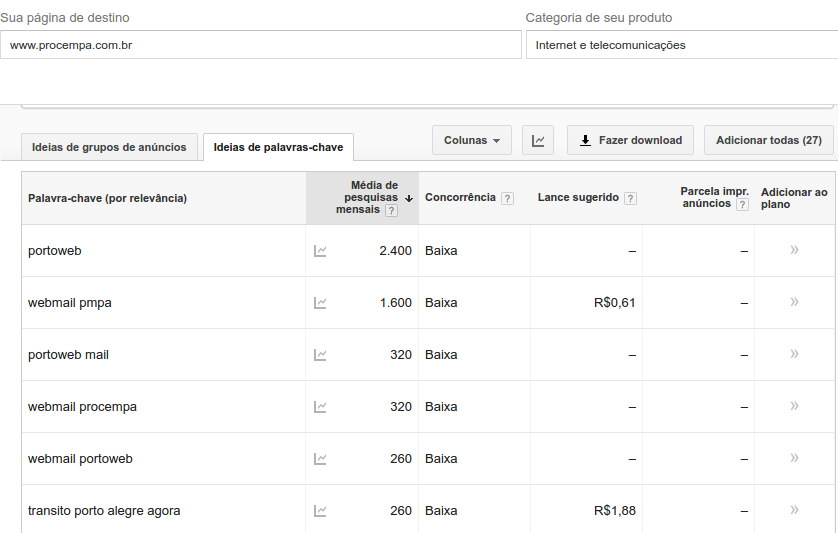
\includegraphics[width=.8\textwidth]{busca-site-procempa}
  \caption{Tendências de Busca Site Procempa}
  \label{fig:busca-site}
\end{figure}

Para atrair novos públicos para o site devemos estabelecer novas palavras para nortearem os conteúdos para o público que queremos atingir. Os formadores de opinião devem buscar por boas práticas na gestão pública, assim produziremos artigos para publicizar as ações de gestão ágil de projetos que temos implementado na companhia. Assim, conforme a Figura \ref{fig:gestao-publica}, deveremos promover conteúdos contendo a palavra chave "Gestão Pública" e seus derivados para melhor ranquearmos nas pesquisas.

\begin{figure}[!h]
  \centering
    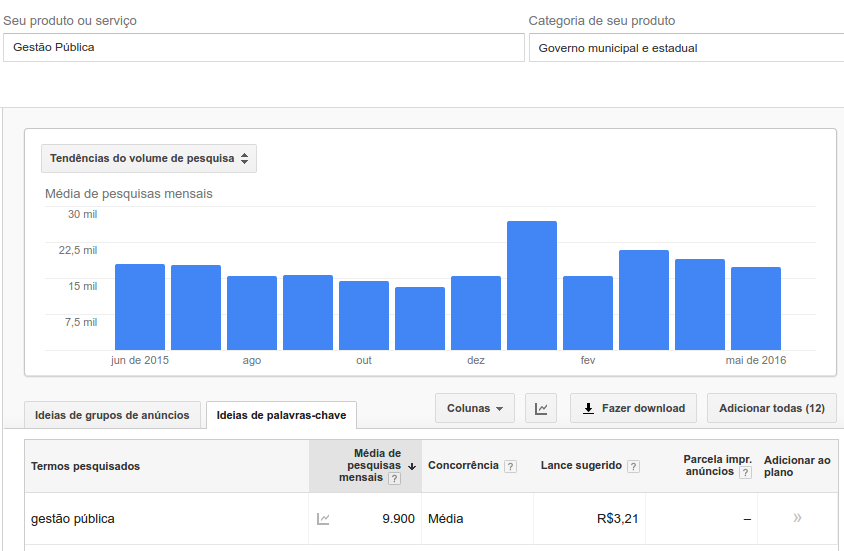
\includegraphics[width=.8\textwidth]{gestao-publica}
  \caption{Palavra Chave Gestão Pública}
  \label{fig:gestao-publica}
\end{figure}

Comunidades de software livre buscarão por iniciativas de código aberto para utilizar em seus próprios projetos. Assim temos que focar em geração de conteúdo útil através do site \citeonline{github} e suas ferramentas como compartilhamento de código e participação em projetos que são parte do dia a dia dos colaboradores. Como vemos na Figura \ref{fig:github-procempa}, atualmente a Companhia possui somente um repositório, já com 8 estrelas mesmo sem nenhum foco de divulgação.

\begin{figure}[!h]
  \centering
    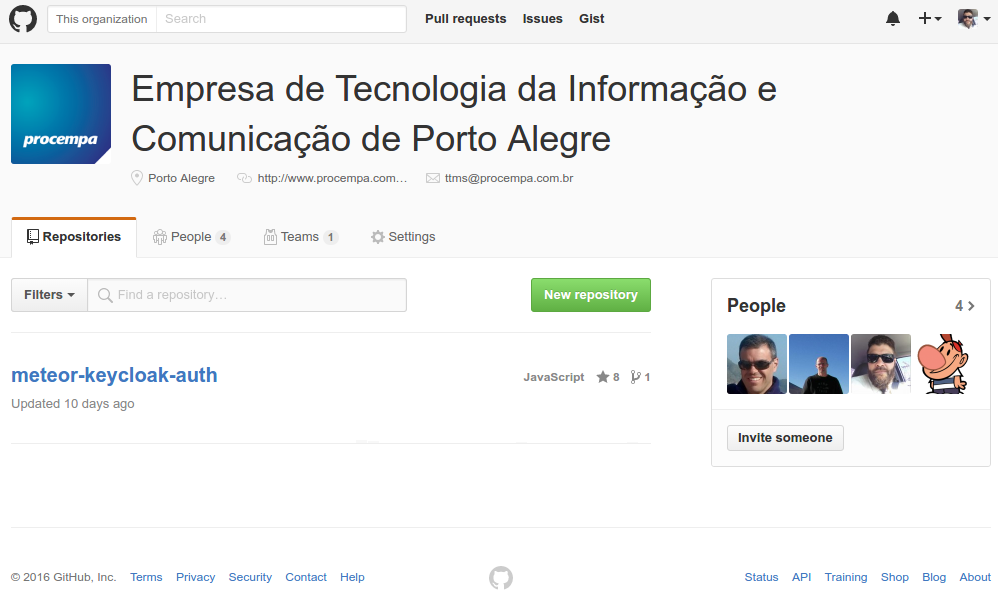
\includegraphics[width=.8\textwidth]{github-procempa}
  \caption{Repositório de Código Procempa no GitHub}
  \label{fig:github-procempa}
\end{figure}

O cidadão da cidade busca por serviços e informações sobre a transparência no trato da coisa pública. Para este público focaremos na parte dos serviços ao cidadão. Como um dos principais serviços com impacto e atendimento direto ao morador ou visitante da cidade, os acessos gratuitos à internet através do \citeonline{poa-livre}, para melhor divulgar esta estratégia o foco será na palavra "Wifi Grátis", conforme as projeções da Figura \ref{fig:wifi-gratis}.

\begin{figure}[!h]
  \centering
    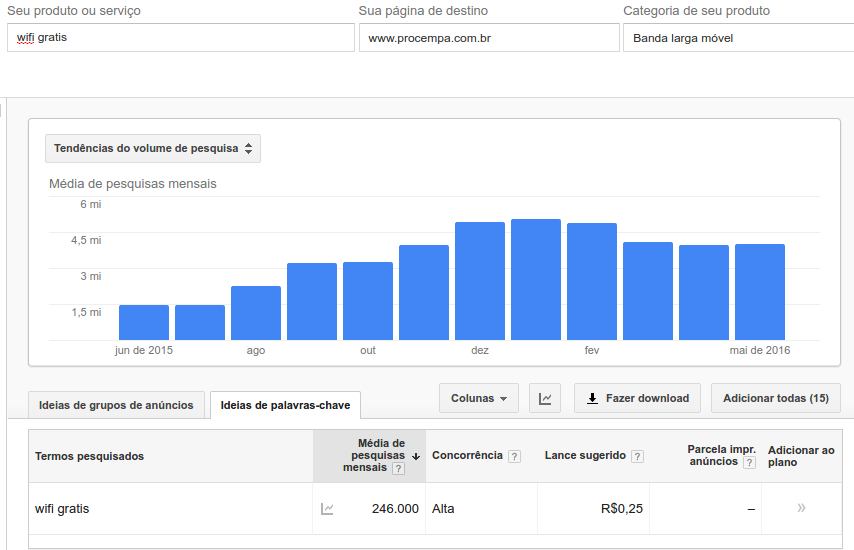
\includegraphics[width=.8\textwidth]{wifi-gratis}
  \caption{Tendências da Palavra Chave Wifi Grátis}
  \label{fig:wifi-gratis}
\end{figure}


\chapter{Planejamento}
Visando atingir os objetivos propostos apresenta-se um planejamento
de atividades a ser realizado no âmbito da Procempa. Estas atividades e o cronograma estão ilustrados nas tabelas \ref{tb:atividades} e
\ref{tb:cronograma}, respectivamente.

%%%% INICIO ATIVIDADES PREVISTAS %%%%%%%%%%%%%%%%%

\begin{table}[!htb]
  \centering
  \caption{Atividades Previstas}\label{tb:atividades}
  \begin{tabular}{cp{12cm}}
    \hline \hline &\\[-0.4cm]
    \textbf{Atividades} & \textbf{Descrição} \\
    \hline
    &\\[-0.4cm]
    \textbf{A} & Apresentação do Planejamento. \\[0.2cm]
    \textbf{B} & Criação das estruturas levantadas pela pesquisa.\\[0.2cm]
    \textbf{C} & Produção de conteúdo.\\[0.2cm]
    \textbf{D} & Monitoria dos resultados. \\[0.2cm]
    \textbf{E} & Divulgação de resultados.\\[0.2cm]
    \hline \hline
  \end{tabular}
\end{table}

%%%% FIM ATIVIDADES PREVISTAS %%%%%%%%%%%%%%%%%

\begin{table}[!htb]
  \centering
  \caption{Cronograma}\label{tb:cronograma}
  \begin{tabular}{cp{1.3cm}p{1.3cm}p{1.3cm}p{1.3cm}p{1.3cm}p{1.3cm}p{1.3cm}}
    \hline \hline &\\[-0.4cm]
    \textbf{Atividades} & Ago/16 & Set/16 &  Out/16 & Nov/16 & Dez/16 \\
    \hline &\\[-0.4cm]
    \textbf{A} & \cellcolor{black!25} &   &   &   & \\[0.2cm]
    \textbf{B} & \cellcolor{black!25} & \cellcolor{black!25} &   &   & \\[0.2cm]
    \textbf{C} &   &  \cellcolor{black!25} & \cellcolor{black!25} & \cellcolor{black!25} & \cellcolor{black!25} \\[0.2cm]
    \textbf{D} &   &  & \cellcolor{black!25} & \cellcolor{black!25}  & \cellcolor{black!25} \\[0.2cm]
    \textbf{E} &   &    &   &  & \cellcolor{black!25}  \\[0.2cm]
    \hline \hline
  \end{tabular}
\end{table}


\chapter{Produção}

O foco da produção de conteúdo pela Procempa serão conteúdos relevantes à comunidades de desenvolvedores de sistemas, preferencialmente livres, focados na solução de problemas comunitários e melhorias nos processos de construção de \emph{software}.
Este conteúdo será gerado pelos colaboradores da companhia, levando em consideração as diretrizes fixadas no manual de comunicação, que serão estimulados por campanha de \emph{endomarketing}. Esta campanha será divulgada através da intranet da empresa, e-mail institucional e quadros existentes na companhia.
Serão disponibilizadas três canais de comunicação, que serão o sítio http://github.com/procempa para compartilhamento de código, o sítio http://stackoverflow.com para auxílio na resolução de dúvidas de outros desenvolveres além de blogs pessoais vinculados à companhia, como por exemplo: http://www.procempa.com.br/blogs/derotino.junior.

\section{Compartilhamento de Código Livre}
O sítio GitHub é um repositório de código aberto, utilizado por mais de trinta e oito milhões de projetos ao redor do mundo. Grandes comunidades de software livre tem seus fontes hospedados nesta plataforma.
A criação de conteúdo neste sítio se dará por dois métodos:

\subsection{Criação de Repositórios Procempa}
A criação de repositórios próprios da Procempa será com trechos reutilizáveis de projetos que não interfiram em sigilo da Prefeitura ou que exponham vulnerabilidades de segurança.

Estes projetos tem que ter sentido fora da estrutura de projeto e ter documentação básica necessária para sua utilização. A publicação dos mesmos deverá ser precedida de alinhamento com as divisões de apoio de tecnologia e componentização do departamento de sistemas.

\subsection{Bifurcação de Projetos}
Com a estratégia de apoio e devolução das colaborações que a Procempa recebe através de códigos livre utilizados, os colaboradores devem ser estimulados a bifurcar projetos de software livres que estiverem utilizando no âmbito de suas tarefas para proposição de melhorias e correções.

\section{Resolução de Dúvidas}
O sítio StackOverflow direciona-se a ser um repositório de perguntas e respostas a cerca do desenvolvimento de software nas mais diversas tecnologias. A cada resposta, ou validação de uma dada por outro participante, o usuário adquire pontos e medalhas que o estabelecem como referencial em uma tecnologia. Esta estratégia, também conhecida como \emph{gamification}, acaba por gerar grande engajamento dos desenvolvedores. A estratégia é estimular aos colaboradores a criarem perfis profissionais e o utilizarem para interagir com o sítio, criando conteúdos relevantes para a comunidade das tecnologias utilizadas na empresa.

\section{Blogs Pessoais}
Deve-se estimular os colaboradores para que mantenham atualizados blogs pessoais relatando novidades e dificuldades encontradas no dia a dia dos projetos. Compartilhar formas de otimização de processos, sistemas e outros assuntos relativos aos interesses da companhia.

Estes conteúdos devem ser orientados a melhorar o ranqueamento das páginas em mecanismos de busca, como o Google, além de serem referências para pesquisas de cidadãos e empresas interessadas nas tecnologias em uso pela Procempa.


\chapter{Publicação}

Nesta função do marketing digital visamos definir a estratégia de publicação do conteúdo gerado. Assim os blogs deverão ser disponibilizados para o público com um frequência a ser definida por cada colaborador, mas monitorada pela gestão de conteúdo da companhia, hoje de responsabilidade da comunicação social.
Em um intervalo mensal serão divulgados os números das ações da Procempa para o público interno e clientes, com a relevância da mesma no cenário de atuação.

Os endereços da Procempa nos sites de conteúdo, definidos anteriormente, deverão ser divulgados no sítio principal da companhia, além dos indicadores de relevância obtidos em cada um dos mesmos. No mesmo sítio deverão ser disponibilizados as ligações para os blogs dos colaboradores com suas biografias profissionais e conteúdos abordados.


\chapter{Promoção}

No cenário de redução de custos atualmente vigente em todos os municípios da federação, a Procempa também tem feito sua parte com melhorias de gestão e contingenciamento de despesas. Assim este planejamento não proporá campanhas com dispêndio financeiro direto para a companhia.

O foco da promoção será estratégias para melhorar a otimização em mecanismos de busca para ganho de pontuação orgânica, sem a necessidade de campanhas pagas para tal. Além destas otimização a relevância dos conteúdos postados nos sítios elencados anteriormente neste plano levarão a companhia a um excelente posicionamento utilizando-se da propaganda do boca-a-boca.


\chapter{Propagação}

A propagação visa atrair nosso público alvo para as redes de colaboração que intentamos montar. Para este fim contaremos com a página oficial da empresa no Facebook que terá publicações contantes de conteúdo gerado pela companhia nos outros meios, além da divulgação dos blogs de colaboradores. O Twitter, por requerer alocação de pessoas de forma mais intensa para sua utilização não será utilizado neste primeiro planejamento.

Serão geradas \emph{releases} de imprensa mensais, a serem disponibilizadas na sala de imprensa do sítio institucional da companhia, com os principais feitos nas mídias propostas por este plano e a relevância destes para os cidadãos.

A participação de colaboradores como palestrantes em eventos de comunidades de software livre, como o Fórum Internacional de Software Livre, deve ser incentivada e as mensagens a serem transmitidas devem estar de acordo com este planejamento e o conteúdo gerado pelo mesmo no seu blog pessoal.


\chapter{Personalização}

Neste item do planejamento estão previstas a possibilidade de assinatura de conteúdo publicados nos blogs, bem como a de anúncios da empresa. Assim devemos ter uma frequência mensal de envio de informações, de acordo com a solicitação dos usuários, para cada público conforme a relevância para estes.

Estes conteúdos devem ser produzidos pela Divisão de Comunicação Social juntamente com as áreas de apoio do Departamento de Sistemas, com conteúdos personalizados para cada público e chamamentos para ações da companhia e divulgação de dados que permitam a fiscalização da comunidade dos atos praticados no âmbito do Departamento.


\chapter{Precisão}

Os resultados das estratégias apontadas neste planejamento serão monitoradas através da ferramenta de análise de dados do Google, \emph{Google Analytics}, assim medindo os resultados de cada conteúdo gerado e sua colocação em relação aos demais. A partir destes dados serão tomadas ações contínuas de melhoria e fomento de informações mais relevantes para nossos públicos.


\chapter{Conclusão}

O momento indica que desenvolver software passa a ser um exercício de criação, muito mais do que técnica, e a computação passa a ser um meio e não o fim. O computador e todo seu poder de processamento, passa a ser ferramenta, assim como o cinzel na mão de Michelangelo. Para que a mente tenha esta capacidade de criação é fundamental que a liberdade e a responsabilidade sejam cláusulas pétreas nas equipes e a comunicação e acesso a informação estejam no centro das estratégias.

A proposição para este cenário é o estudo da arte de desenvolver aplicações de alto valor agregado, escaláveis e confiáveis, sendo feliz durante sua construção. Para isto precisamos colocar os valores humanos sempre em primeiro lugar, investir fortemente em formação técnica, tendo em mente que essa é apenas o meio nunca o fim, buscar qualificação emocional e, principalmente, buscar o  que nos faz feliz. Sabe-se que as dificuldades do caminho não são pequenas, mas a persistência, foco e treinamento nos levarão a construir nosso próprio David, trazendo à vida aplicações úteis e que possam agregar valor à sociedade e satisfação ao seu criador.

Neste planejamento buscamos demonstrar como o empoderamento dos colaboradores pode melhorar sua produtividade e alavancar a Companhia ao patamar de referência em construção de software e processos. A base de tudo o que precisamos para isto já está disponível em larga quantidade de patrimônio intelectual gerado a cada dia pelas equipes. Assim somente precisamos apor os trilhos para que essa grande locomotiva de conhecimento possa acelerar resultados tangíveis para todos, sejam eles a Prefeitura, os cidadãos ou as comunidades de software.


\postextual

\bibliography{projeto-marketing-procempa-referencias}

\phantompart

\printindex

\end{document}
